\section{Benutzungsoberfläche}
\subsection{Allgemeiner Aufbau}
 In den Abbildungen \ref{ui-max} und \ref{ui-min} wird der  Entwurf des Hauptnutzerinterface gezeigt. Generell betrachtet ist die Oberfläche in zwei Bereiche geteilt. Im oberen Abschnitt befindet sich der Kopfbereich. Dieser stimmt in allen für den Endnutzer bestimmten Anwendungsbereichen überein. Darunter liegt eine für die einz
 Der Bereich mit den zusätzlichen Informationen(8) kann ausgeblendet werden. Dadurch steht für andere Bereiche der Anwendung mehr Platz zur Verfügung. Insbesondere bei kleineren Anzeigegeräten wie Tablets oder anderen mobilen Geräten kommt dieser Fakt zum Tragen. 
 
 
 
\subsection{Bedienelemente}
 \begin{enumerate}
 	\item 
 \end{enumerate}
 
\begin{figure}[ht]
 
 	\centering
 	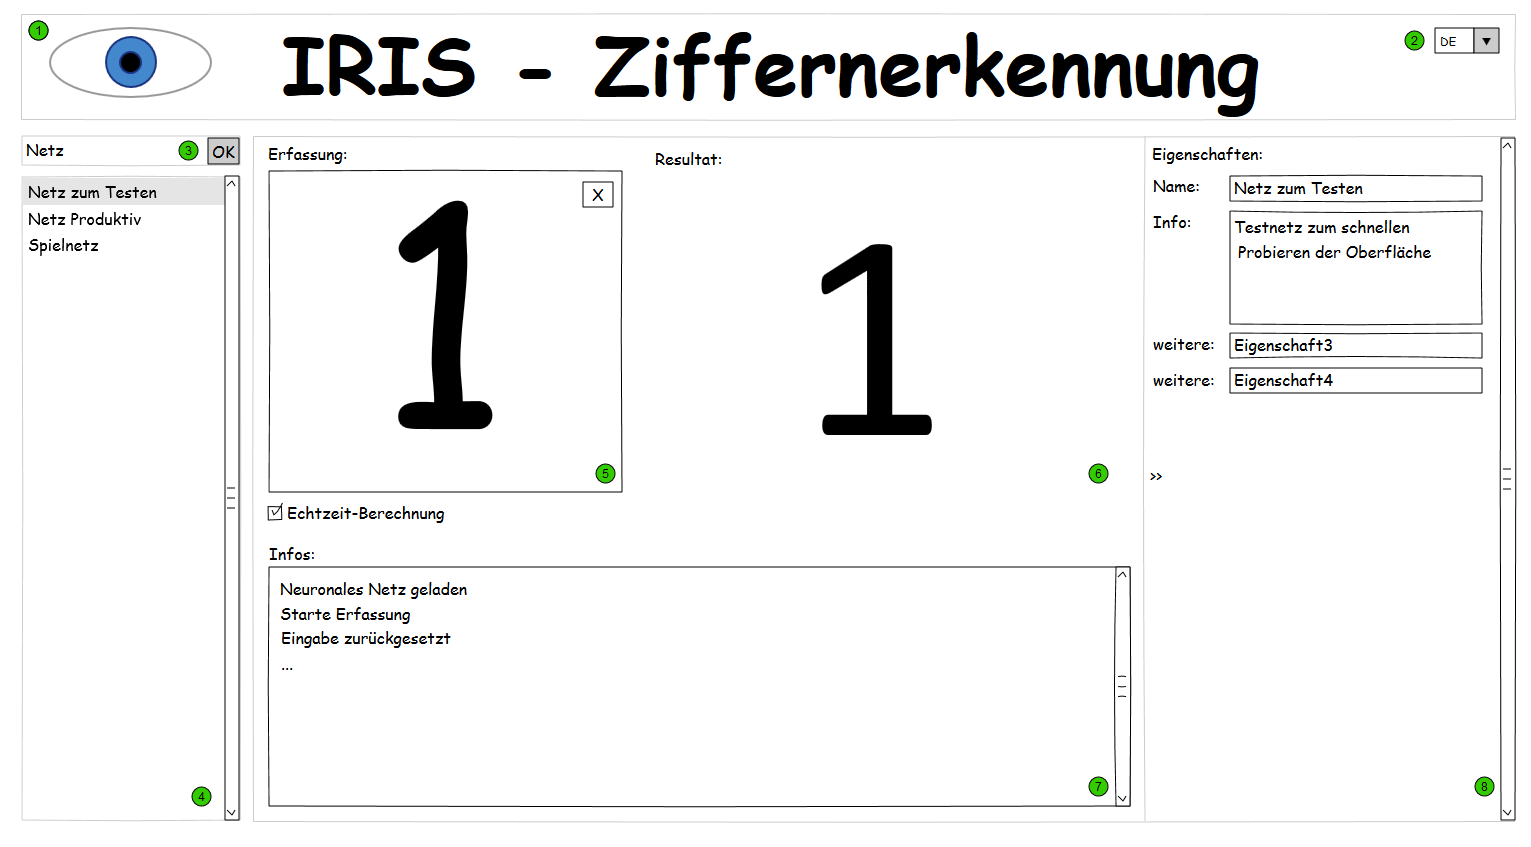
\includegraphics[height=0.8\textwidth, angle=90]{Abbildungen/UI-Mocks/Main-Ui.png}
 	\caption{Nutzeroberfläche mit eingeblendeten Metainformationen}
 	\label{ui-max}
\end{figure}

\begin{figure}[ht]
	\centering
	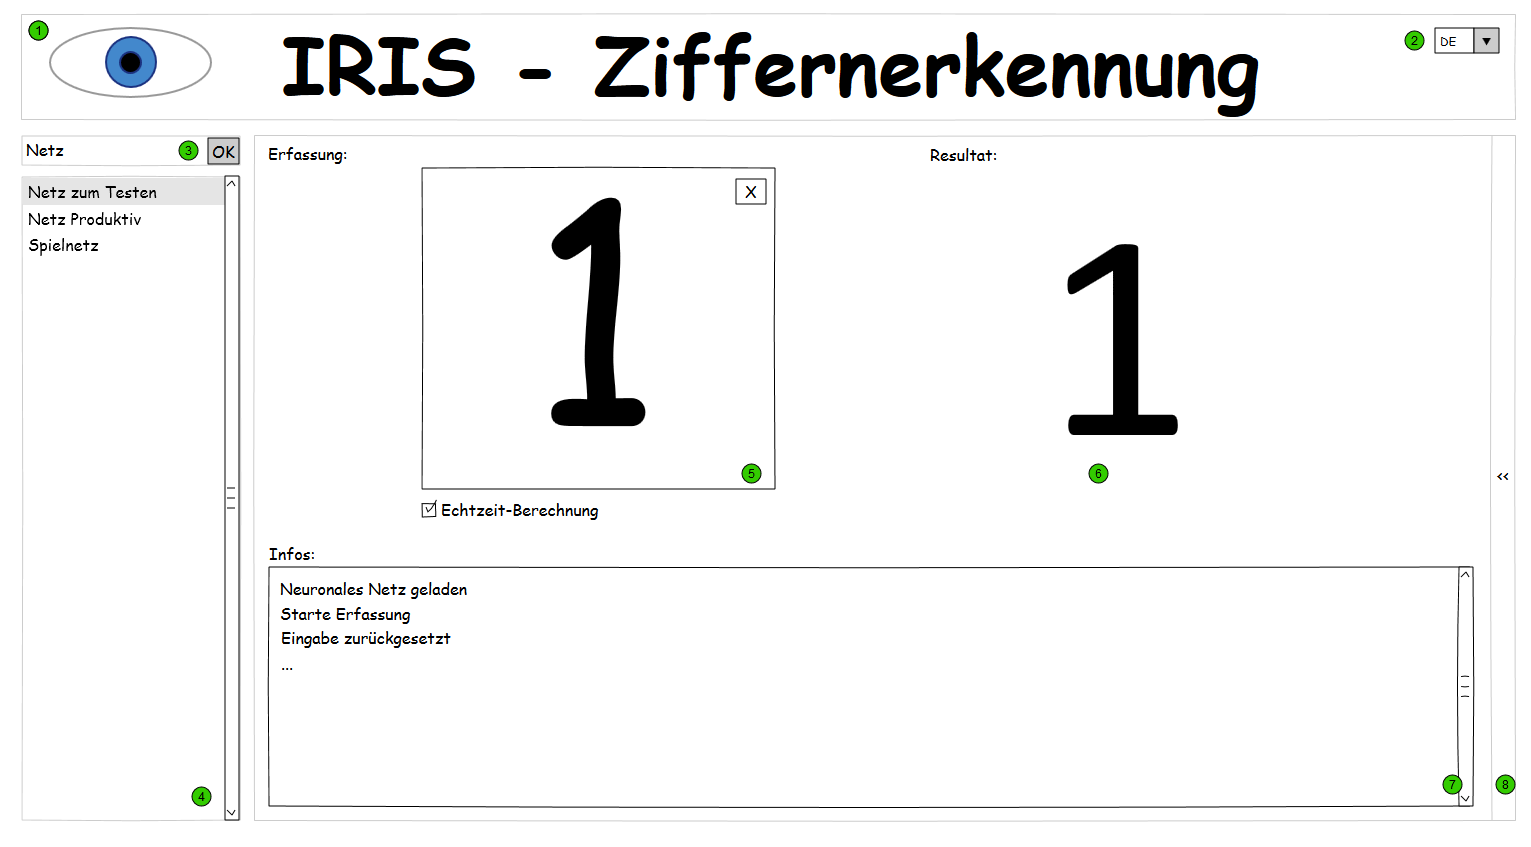
\includegraphics[height=0.8\textwidth, angle=90]{Abbildungen/UI-Mocks/Main-Ui-Minimized.png}
	\caption{Nutzeroberfläche mit ausgeblendeten Metainformationen}
	\label{ui-min}
\end{figure}

%Benutzungsoberfläche: grundlegende Anforderungen, Zugriffsrechte
